% \begingroup
% \let\clearpage\relax 
% \onecolumn

%\vspace{20mm}

Figure \ref{fig:dataset_partition} presents one time-series for each dataset and the train, validation, and test splits. Table \ref{table:datasets_summary} presents summary statistics for the benchmark datasets.

\begin{figure}[!ht] %t+*
\centering     %%% not \center
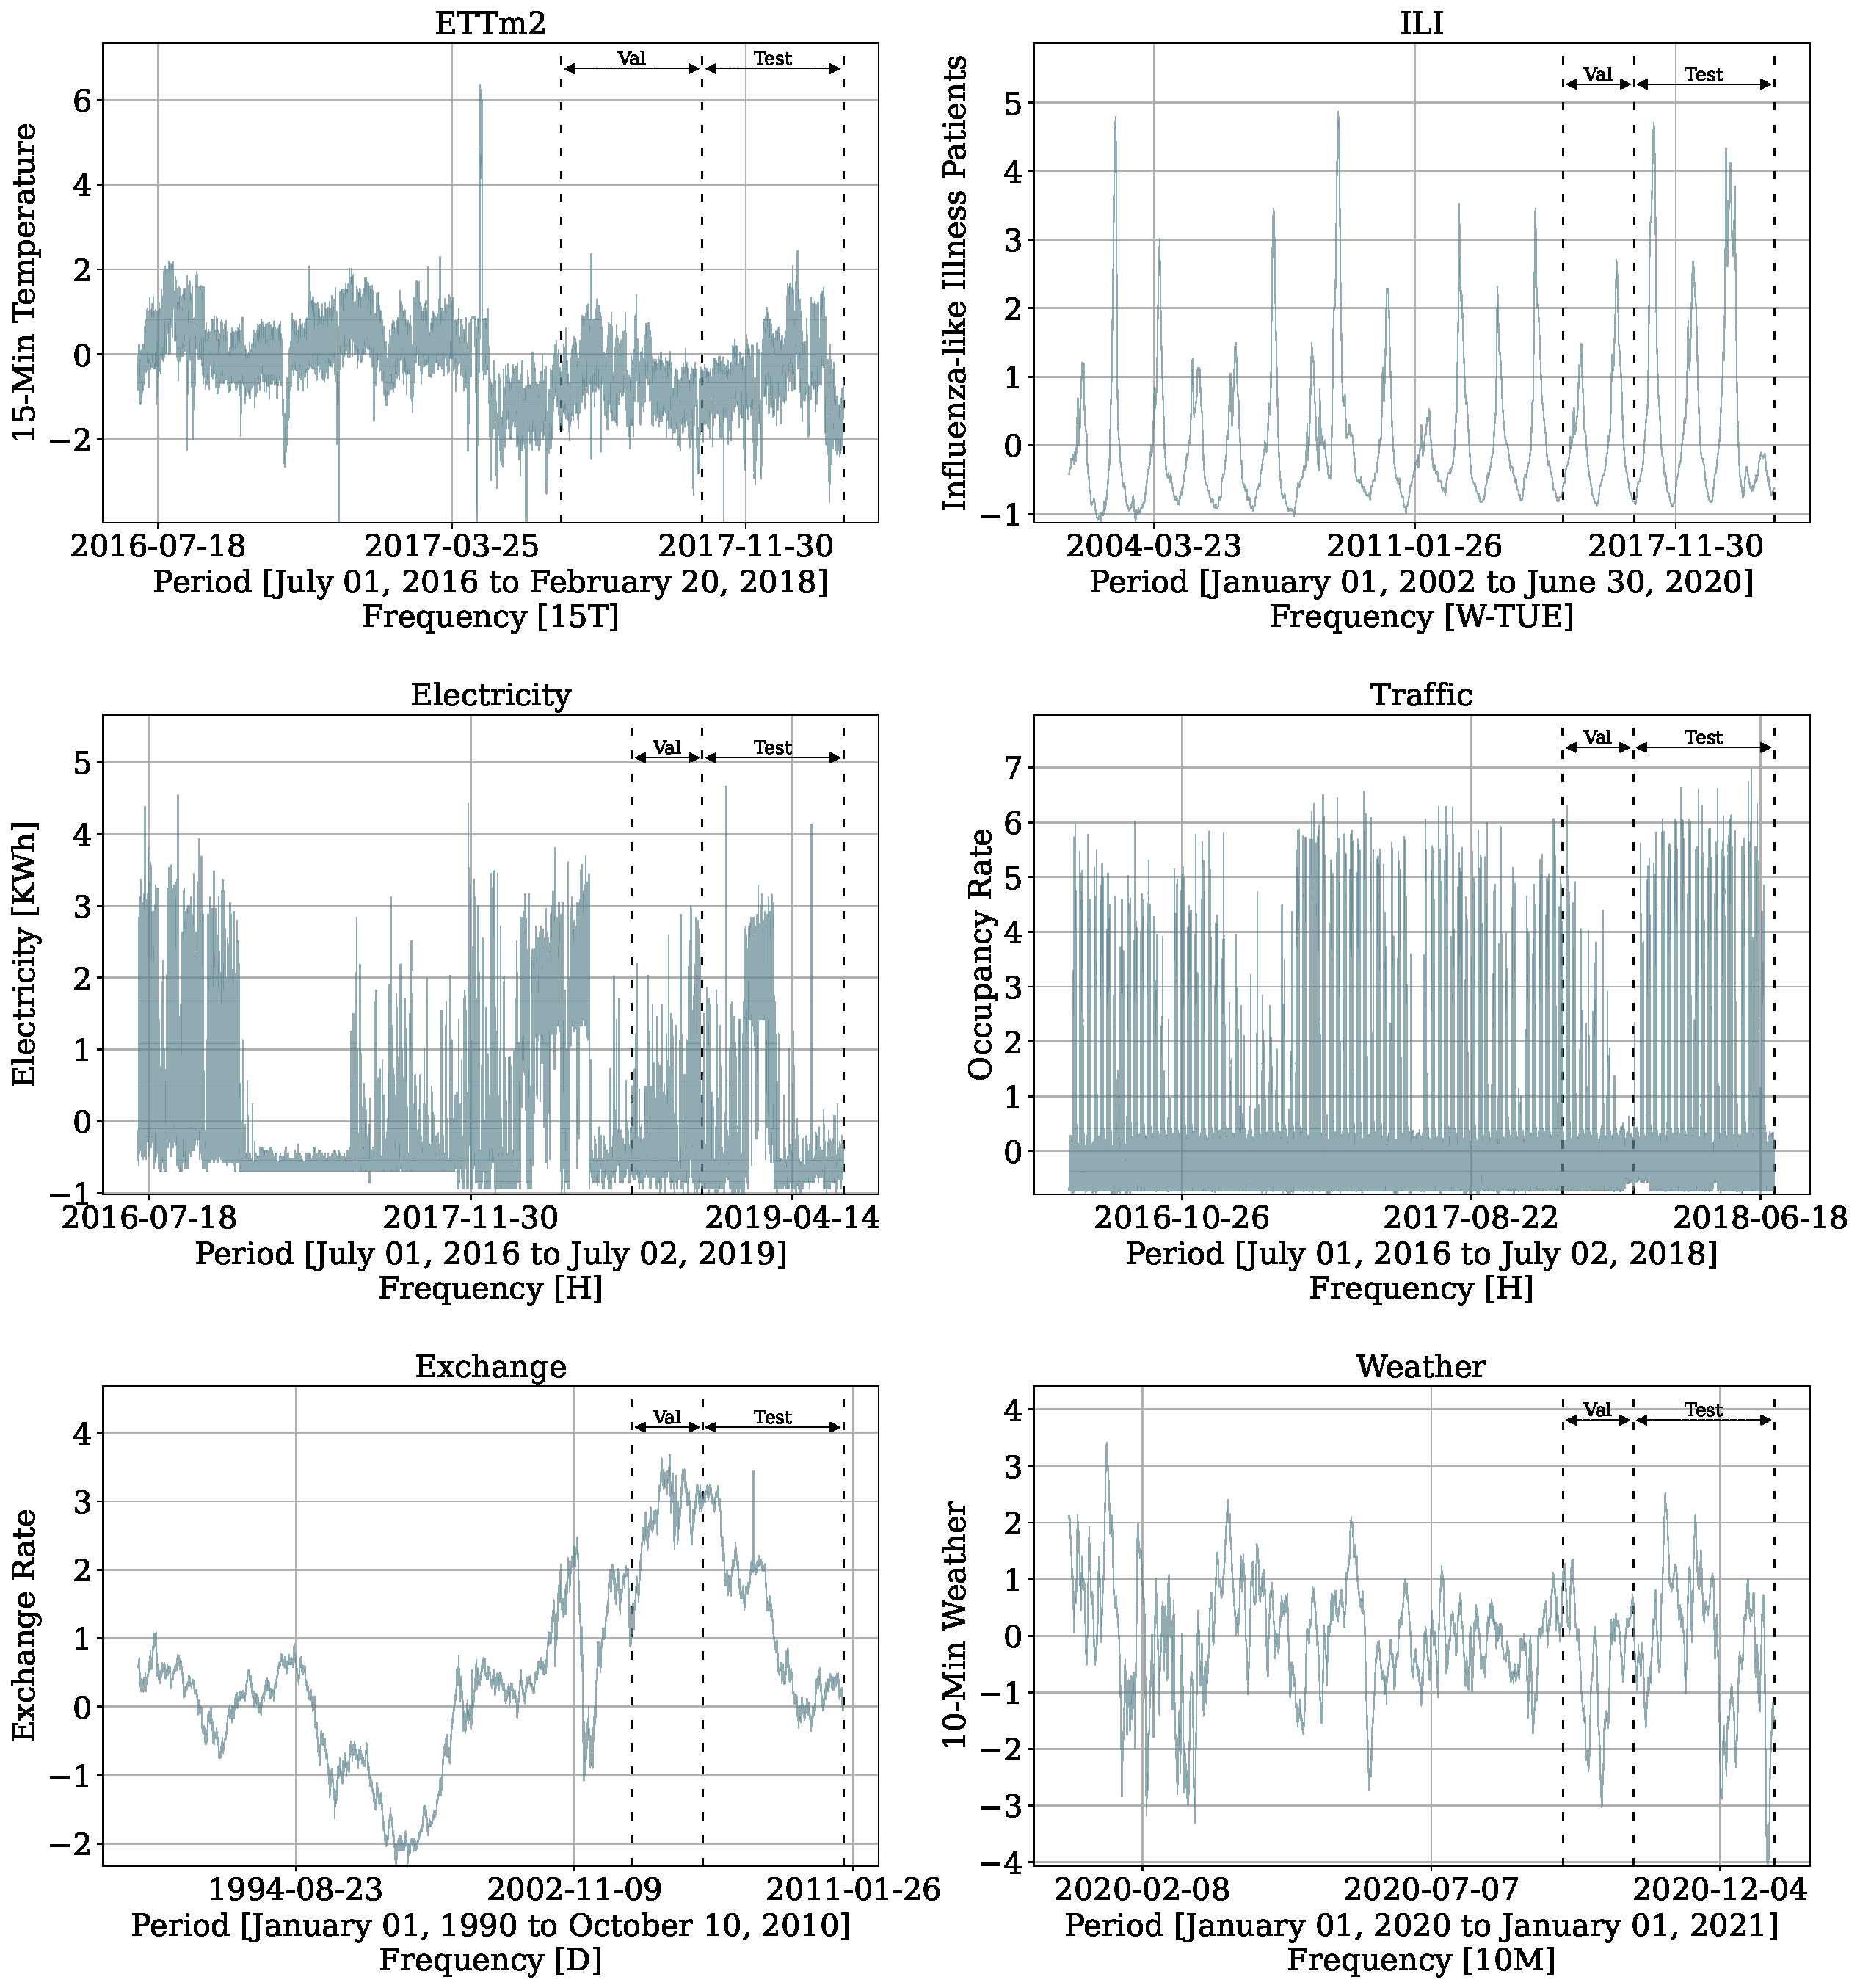
\includegraphics[height=9.3cm]{images/plot-graphs-dmidas.pdf}
\caption{Datasets' partition into train, validation, and test sets used in our experiments (\ETTm$_2$, \Electricity, \Exchange, \ILI, \TrafficL, and \Weather). All use the last 20\% of the total observations as test set (marked by the second dotted line), and the 10\% preceding the test set as validation (between the first and second dotted lines), except for \ETTm$_2$ \ that also use 20\% as validation. Validation  provides the signal for hyperparameter optimization. We construct test predictions using rolling windows.}
\label{fig:dataset_partition}
\end{figure}

% \endgroup

